\section{Development View}

Im Folgenden wird die Sicht auf die Anwendung während der Entwicklung beschrieben.

\subsection{Software Components}

\subsubsection{Source code organization}
Für die Organisation unseres Quellcodes haben wir einen Monorepo-Ansatz verwendet. Alle Backend-Services, das Frontend und die Dateien für CI/CD sind in diesem Repository in der Ordnerstruktur wie in Figure \ref{fig:repo-structure} gezeigt abgelegt.

\begin{figure}[ht]
    \begin{verbatim}
        park
        |-- backend
        |   |-- authentication
        |   |   |-- ...
        |   |-- infrastructure-administration
        |   |   |-- ...
        |   |-- parking-management
        |   |   |-- ...
        |   |-- property-management
        |   |   |-- ...
        |   |-- shared
        |-- certs
        |-- ci-cd
        |   |-- helm
        |   |   |-- ...
        |   |-- terraform
        |       |-- ...
        |-- cloud-functions
        |-- docs
        |   |-- ...
        |-- frontend
        |   |-- ...
        |-- shared
        |-- signup-frontend
        |-- ...
    \end{verbatim}
    \caption{Repository Structure}
    \label{fig:repo-structure}
\end{figure}

Für alle einzelnen Backend Microservices existiert unter \verb|backend| ein Unterordner, in dem das Node.js Projekt des entsprechenden Microservices abgelegt ist. Zusätzlich sind unter \verb|shared| TypeScript files abgelegt, die von mehreren Backend Services verwendet werden.

Der Ordner \verb|certs| ist für das lokale Testing, um dort die Key-Files der Service Accounts abzulegen.

In \verb|ci-cd| sind alle Dateien für DevOps und das Deployen der Infrastruktur abgelegt. Unter \verb|helm| liegen dabei alle Dateien, die für das Erstellen der Helm Charts benötigt werden, \verb|terraform| beinhaltet alle Konfigurationsdateien für die Cloud-Infrastruktur. Außerdem befinden noch Python-Skripte für das Deployment-Handling in diesem Verzeichnis.

Damit auch der Code für die Cloud-Functions in die Quellcodeverwaltung aufgenommen sind, existiert für diese das \verb|cloud-functions| Verzeichnis.
Unter \verb|docs| liegen einige Files für die Dokumentation ab. Darunter Skizzen für die API-Spezifikation.

Im \verb|frontend| Verzeichnis befindet sich der gesamte Client-Code der Anwendung, in diese Fall ein React Projekt mit allen Komponenten und Services des Frontends.
Außerdem existiert noch ein weiteres \verb|shared| Verzeichnis auf top-level Ebene für die DTOs zwischen Frontend und Backend.

Für die Tenant-Creation, beziehungsweise der Registrierung und Instanzerstellung für neue Tenants existiert noch ein separater Client, welcher unter \verb|signup-frontend| abgelegt ist. Hierbei handelt es sich ebenfalls um ein React-Projekt.

Während der Entwicklung haben wir mit Feature-Branches angelegt an den Git Flow gearbeitet, um eine möglichst konfliktfreie, parallele Entwicklung der Anwendung zu ermöglichen.

\subsubsection{Components}
Die Applikation umfasst 4 Microservices für das Backend:

\begin{itemize}
    \item \textbf{Authentication Service:} Erweiterung der Authentication-Funktionalität für den Kontext der Anwendung
    \item \textbf{Infrastructure Management Service:} Zentrale Verwaltung der Tenant Creation und Endpunkt zur Konsolidierung von Anwendungsweiten Analytics
    \item \textbf{Parking Management Service:} Bereitstellung der gesamten Funktionalität für das Parken, Laden und die Belegungsverwaltung
    \item \textbf{Property Management Service:} Bereitstellung der Gesamten Funktionalität für die Verwaltung der Parkinfrastruktur
\end{itemize}

Zusätzlich werden 2 Frontend Clients bereitgestellt:

\begin{itemize}
    \item \textbf{PARK Client:} Frontend für die Bedienung der Anwendung
    \item \textbf{SignUp Client:} Frontend für die Tenant-Creation/Instanzerstellung
\end{itemize}

Wie bereits im Kontextdiagram (Figure \ref{fig:context-diagram}) gezeigt, sind zudem verschiedene externe Komponenten angebunden. So werden beispielsweise unterschiedliche Komponenten aus der Google Cloud Infrastruktur verwendet (Object Storage, Firestore, Identity Platform,...). Außerdem werden extern verwaltete Komponenten angebunden, beispielsweise in Form von Schranken, Ladestationen usw. Für das automatisierte Deployment werden GitHub Actions verwendet.

\subsubsection{Libraries}
Für die Interaktion mit der Google Cloud Infrastruktur wurden unterschiedliche Libraries verwendet. Für den Zugriff auf die Firestore Infrastruktur haben wir das NPM Paket \href{hhttps://www.npmjs.com/package/firebase-admin}{firebase-admin} verwendet, welches verschiedene Methoden, beispielsweise zum Abrufen und Erstellen von Dokumenten in einer Firestore Datenbank zur Verfügung stellt.

Um Zugriff auf den Object Storage zu haben, um beispielsweise bei der Defect-Erstellung Bilder ablegen zu können haben wir den \href{https://www.npmjs.com/package/@google-cloud/storage}{google-cloud/storage} NPM Client verwendet.

Die Kommunikation mit der Google Cloud Identity Platform für das frontendseitige Anmelden ist über das \href{https://www.npmjs.com/package/@firebase/app-compat}{@firebase/app-compat package} realisiert.

Da für die Authentifizierung der Komponenten innerhalb der Anwendung JWT Tokens verwendet werden, sind außerdem die \href{https://www.npmjs.com/package/jsonwebtoken}{jsonwebtoken} Library und der OAuth2Client Client aus der \href{https://www.npmjs.com/package/google-auth-library}{google-auth-library} eingebunden.

\subsubsection{APIs}
Im Wesentlichen stellt jeder Service eine API bereit, wie in Abbildung \ref{fig:api-overview} dargestellt, über welche dessen Funktionalität genutzt werden kann.

\begin{figure}[ht]
    \centering
    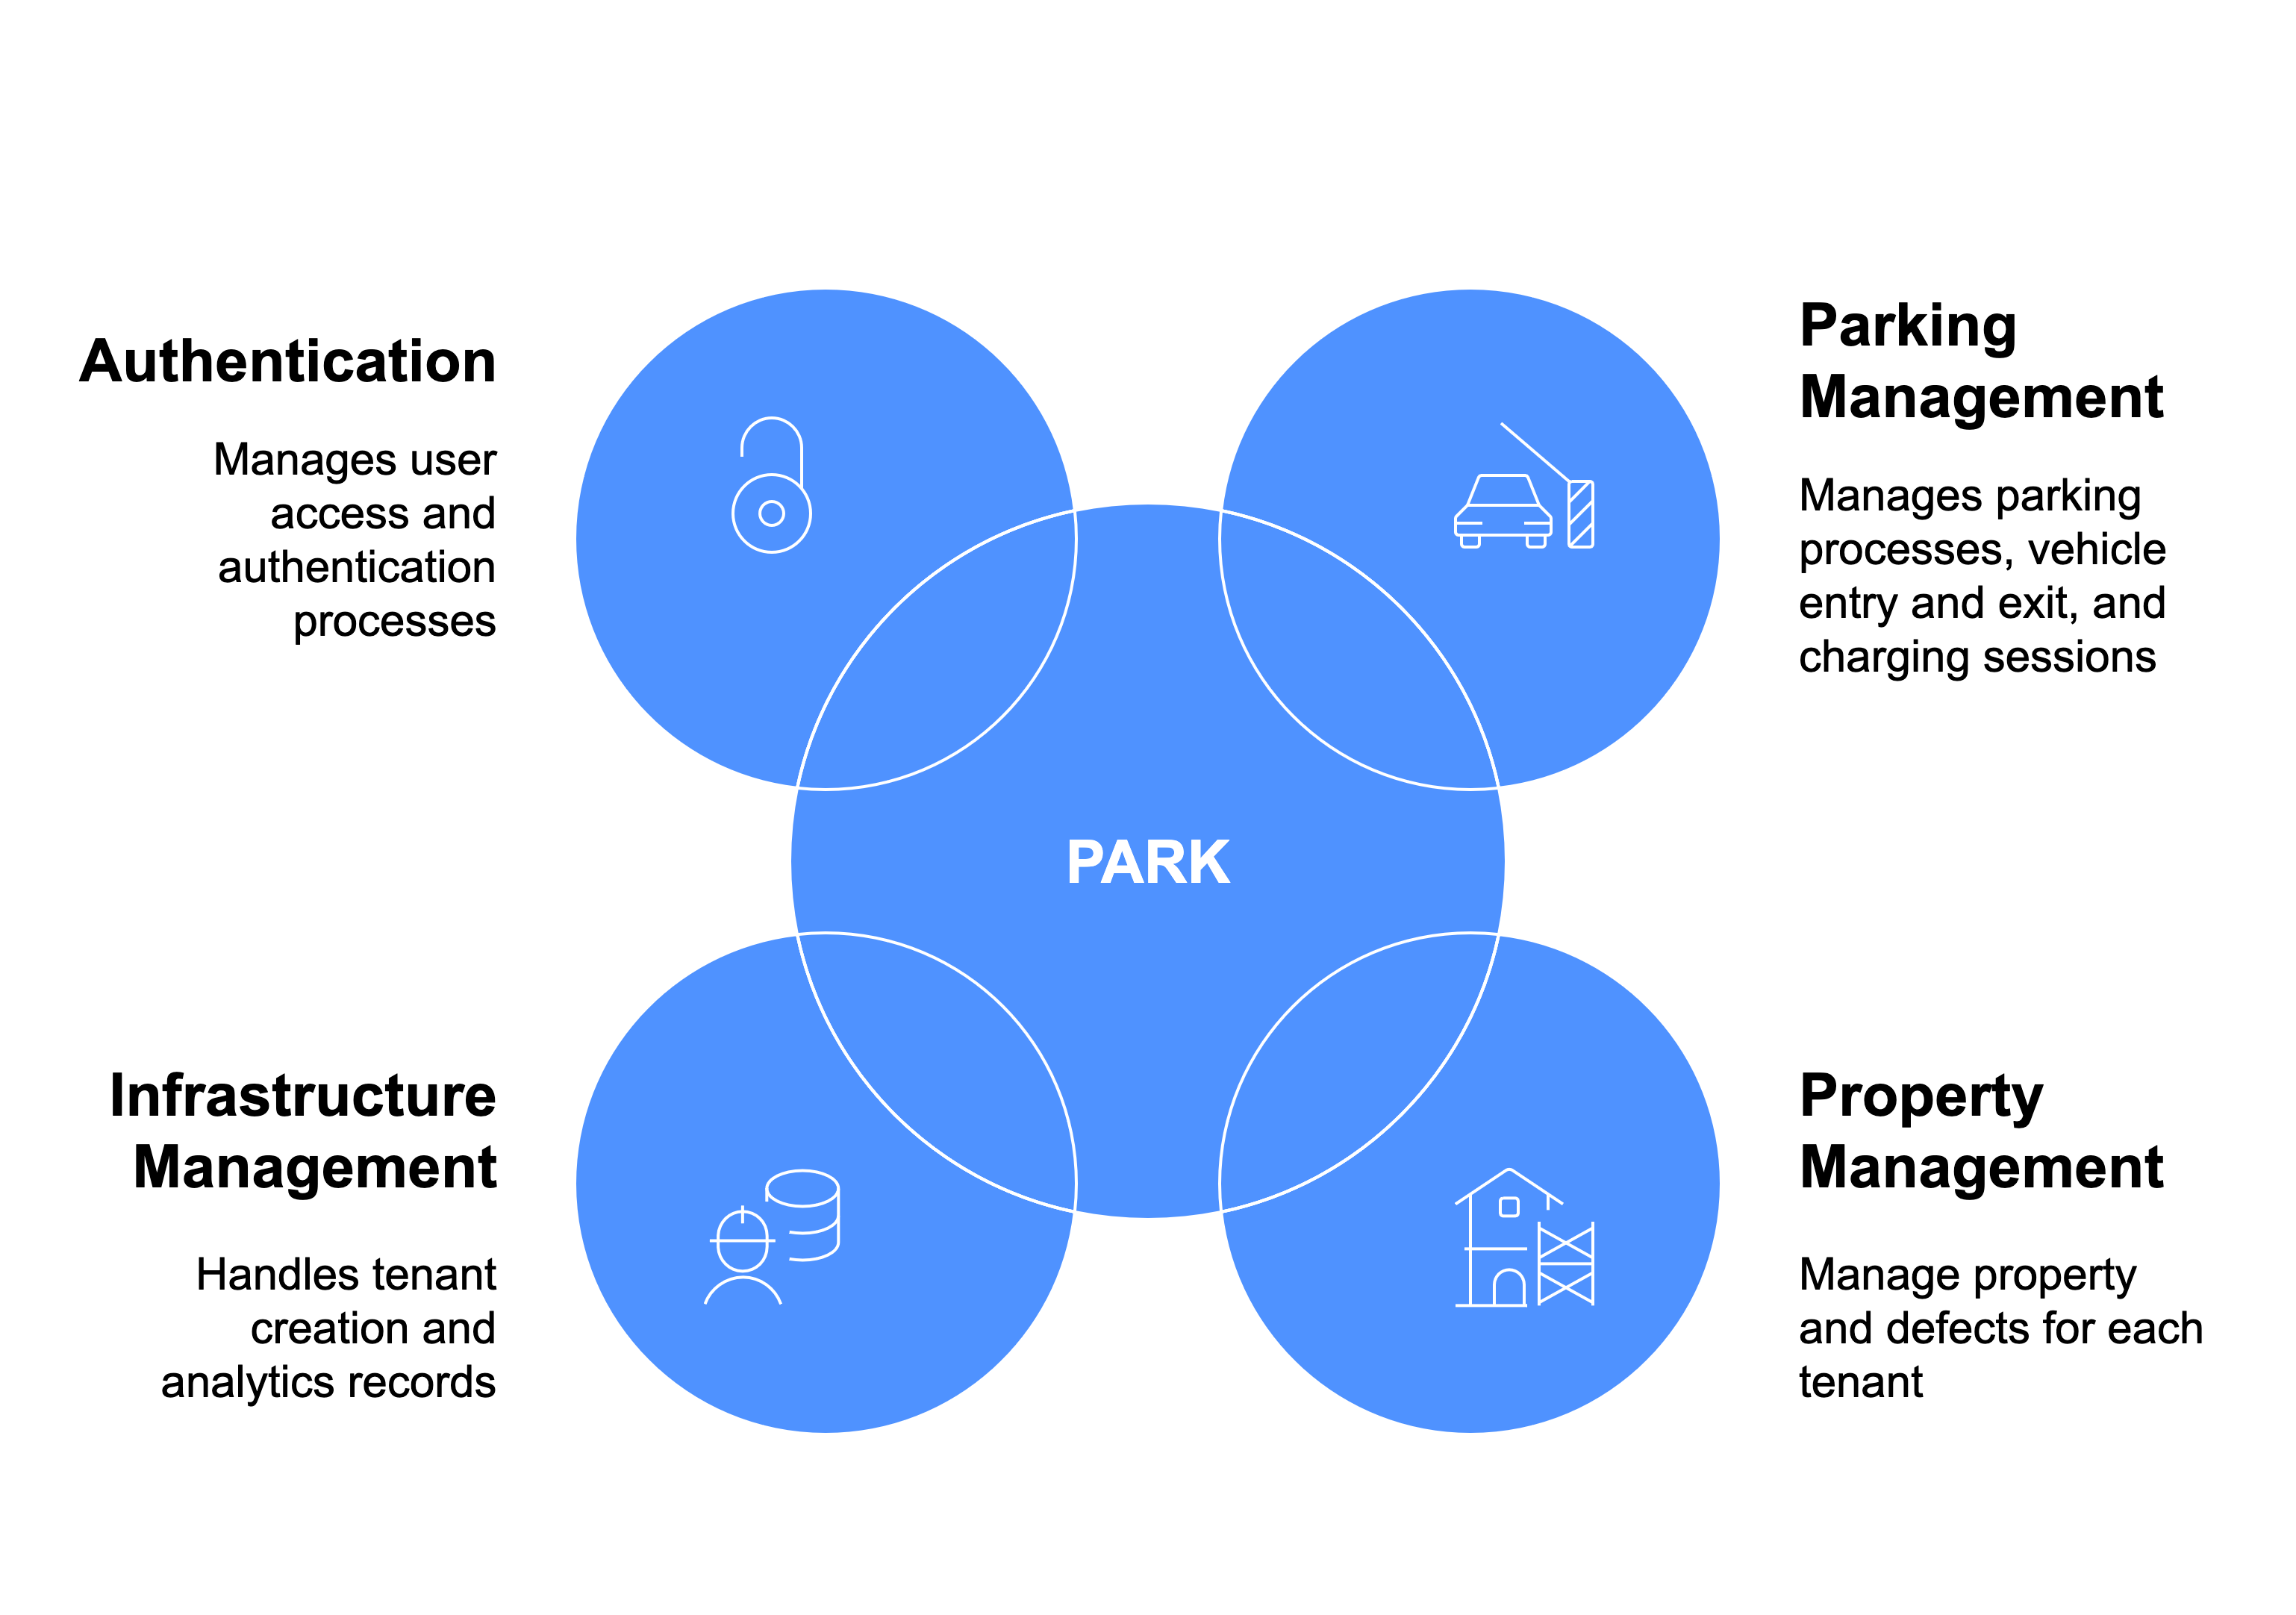
\includegraphics[width=0.9\textwidth]{resources/api-overview-blue.png}
    \caption{Übersicht der APIs}
    \label{fig:api-overview}
\end{figure}

Über die Parking Management API können alle Prozesse, die sich auf die Verwendung der Park- und Ladeinfrastruktur beziehen, verwendet werden. \\

\textbf{Parking Management:}
\begin{itemize}[noitemsep]
    \item[] \verb|GET garage/:garageId|
    \item[] \verb|POST garage/create|
    \item[] \verb|PUT garage/update|
    \item[] \verb|DELETE garage/delete/:garageId|
    \item[] \verb|GET garage/parking/occupancy/:garageId|
    \item[] \verb|GET garage/charging/occupancy/:garageId|
    \item[] \verb|POST garage/enter/:garageId|
    \item[] \verb|POST garage/handlePayment/:ticketId|
    \item[] \verb|GET garage/mayExit/:ticketId|
    \item[] \verb|POST garage/exit/:garageId|
    \item[] \verb|POST garage/charging/startSession/:garageId/:stationId/:userId|
    \item[] \verb|POST garage/charging/endSession/:garageId/:sessionId|
    \item[] \verb|GET garage/charging/session/:sessionId|
    \item[] \verb|GET garage/charging/invoice/:sessionId|
\end{itemize}

Die API des Property Management Services stellt alle Endpunkte für das Erstellen, Bearbeiten und Löschen der Parkhausinfrastruktur bereit. \\

\textbf{Property Management:}
\begin{itemize}[noitemsep]
    \item[] \verb|GET defects|
    \item[] \verb|GET defects/:id|
    \item[] \verb|POST defects|
    \item[] \verb|Put defects/:id|
    \item[] \verb|DELETE defects/:id|
    \item[] \verb|GET defects/signedUrl/:image|
    \item[] \verb|GET defects/signedUploadUrl/:image|
\end{itemize}

Im Infrastruktur Management Service ist die gesamte Analytics Funktionalität gebündelt. Für unterschiedliche Analysen können Records gespeichert werden (beispielsweise Belegung der Park- und Ladeplätze, Parkdauer, Energieverbrauch der Ladeinfrastruktur und Status der Defect-Verwaltung). Abgefragt werden können zumeist entweder die aktuellsten Werte für einen bestimmten Zeitpunkt oder eine Liste von Werten in einem bestimmten Zeitpunkt. Dieser Endpunkt wird beispielsweise für die Erstellung der Histogramme im Frontend verwendet. Der Aufbau dieser Records wird im folgenden Kapitel noch detaillierter beschrieben.
Neben den Analytics Endpunkten stellt der Service auch einen Endpunkt für die Erstellung eines neuen Tenants bereit. \\

\textbf{Infrastructure Management:}
\begin{itemize}[noitemsep]
    \item[] \verb|POST tenants/add|
    \item[] \verb|PUT analytics/parking/status/:tenantId/:garageId|
    \item[] \verb|GET analytics/parking/status/:garageId/:timestamp|
    \item[] \verb|GET analytics/parking/status/:garageId/:start/:end|
    \item[] \verb|PUT analytics/charging/status/:tenantId/:garageId|
    \item[] \verb|GET analytics/charging/status/:garageId/:timestamp|
    \item[] \verb|GET analytics/charging/status/:garageId/:start/:end|
    \item[] \verb|PUT analytics/parking/duration/:tenantId/:garageId/:duration|
    \item[] \verb|GET analytics/parking/duration/:garageId/:start/:end|
    \item[] \verb|PUT analytics/charging/powerConsumed/:tenantId/:garageId/:consumption|
    \item[] \verb|GET analytics/charging/powerConsumed/:garageId/:start/:end|
    \item[] \verb|PUT analytics/turnover/:tenantId/:garageId/:turnover|
    \item[] \verb|GET analytics/turnover/:garageId/:start/:end|
    \item[] \verb|PUT analytics/defects/status/:tenantId/:garageId|
    \item[] \verb|GET analytics/defects/status/:tenantId/:garageId/:timestamp|
    \item[] \verb|GET analytics/defects/status/:garageId/:start/:end|
    \item[] \verb|PUT analytics/requests/:tenantId|
    \item[] \verb|GET analytics/requests/:tenantId/:from/:to|
\end{itemize}

Die Schnittstelle des Authentication Service stellt einige Erweiterungen um die Google Cloud Identity Platform bereit, um beispielsweise Informationen über bestimmte Nutzer abzufragen. \\

\textbf{Authentication:}
\begin{itemize}[noitemsep]
    \item[] \verb|GET user/:userId|
    \item[] \verb|GET all-users|
    \item[] \verb|PUT user|
    \item[] \verb|POST user/:userId|
    \item[] \verb|DELETE user/:userId|
    \item[] \verb|POST tenants/add|
\end{itemize}

\subsection{Data Model}
Verschiedene Datenbanken
Analytics Records
Garage (Parking und Property Management)
Defects (Dokumente und Bilder im object storage)
tickets und charging sessions

